

程序分析和测试一起进行,以确保解决方案的质量。当使用测试代码时,运行Valgrind会变得更加一致。出于这个原因,可以将这两个东西配置在一起。图12.5演示了执行流程和设置它们所需的文件(一些代码片段将添加到src目录):

\begin{center}
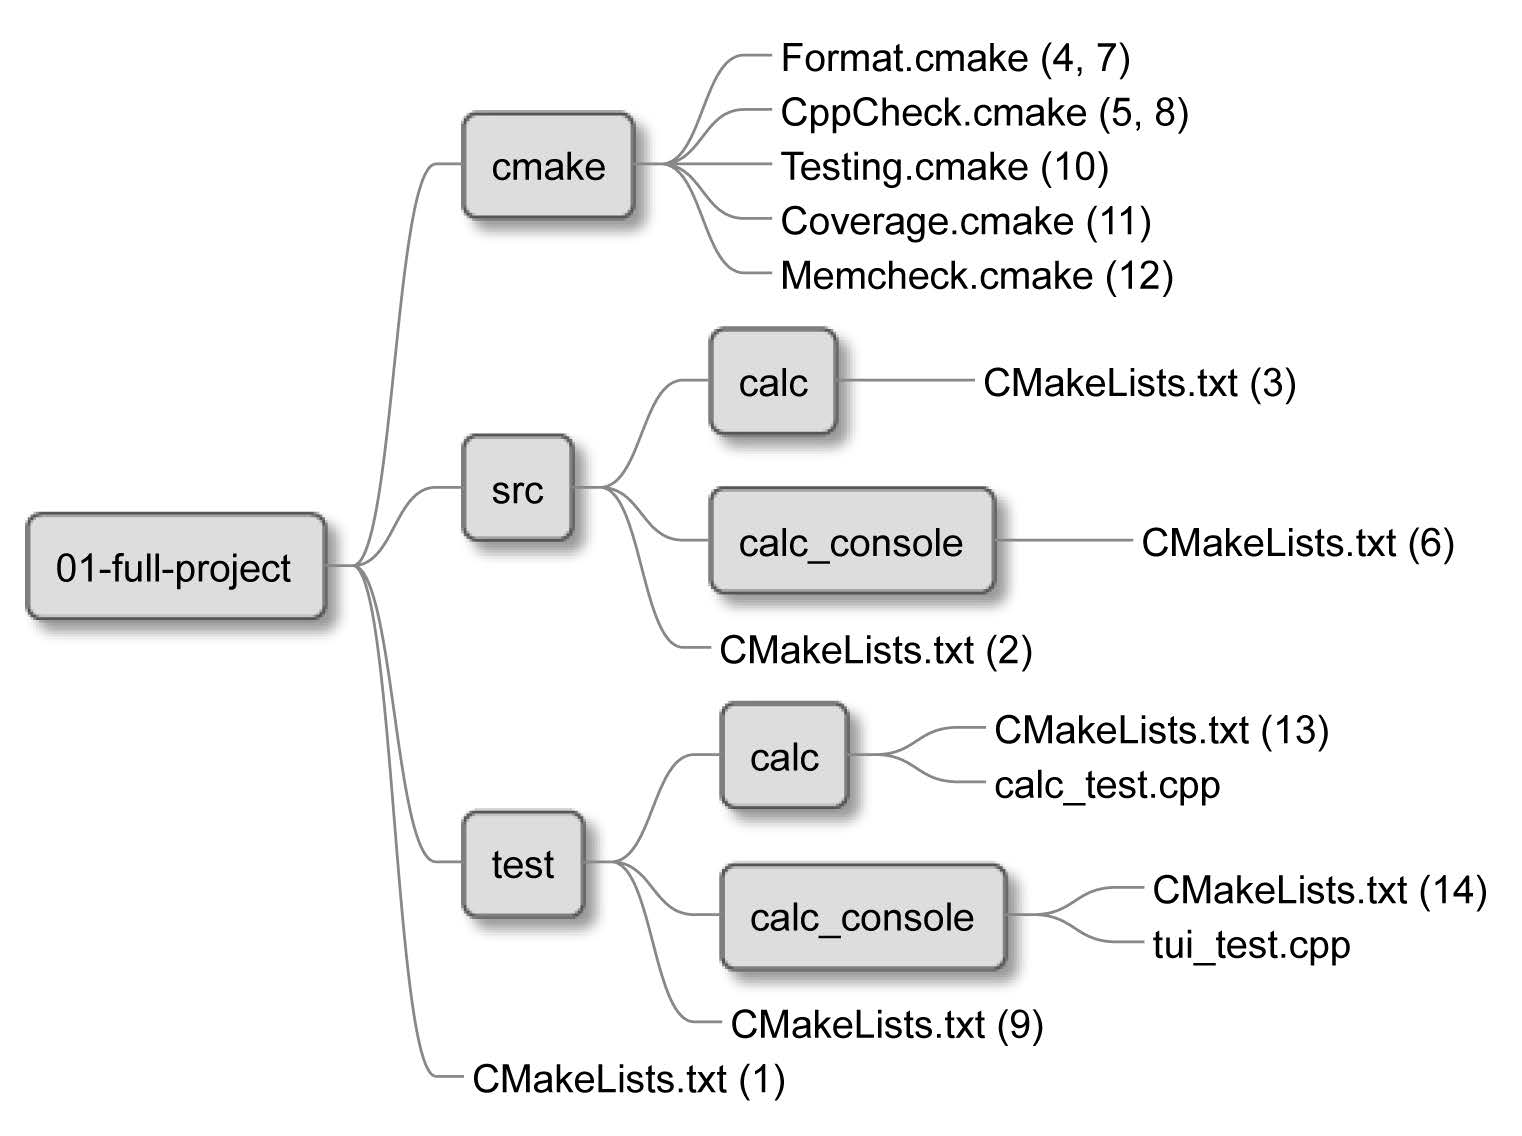
\includegraphics[width=0.6\textwidth]{content/3/chapter12/images/5.jpg}\\
图12.5 启动测试和程序分析
\end{center}

测试位于test目录中,其列表文件通过add\_subdirectory()指令从顶层列表文件中执行。来看看里面有什么:

\begin{lstlisting}[style=styleCMake]
# chapter-12/01-full-project/test/CMakeLists.txt

include(Testing)
add_subdirectory(calc)
add_subdirectory(calc_console)
\end{lstlisting}

Testing模块中定义的测试实用程序包含在这个级别,以允许两个目标组(来自calc和calc\_console目录)使用:

\begin{lstlisting}[style=styleCMake]
# chapter-12/01-full-project/cmake/Testing.cmake (fragment)

enable_testing()
include(FetchContent)
FetchContent_Declare(
	googletest
	GIT_REPOSITORY https://github.com/google/googletest.git
	GIT_TAG release-1.11.0
)
# For Windows: Prevent overriding the parent project's
# compiler/linker settings
set(gtest_force_shared_crt ON CACHE BOOL "" FORCE)
option(INSTALL_GMOCK "Install GMock" OFF)
option(INSTALL_GTEST "Install GTest" OFF)
FetchContent_MakeAvailable(googletest)
...
\end{lstlisting}

启用了测试并包含了FetchContent模块来获取GTest和GMock,这个项目中并没有真正使用GMock,但是这两个框架会捆绑在一个库中,因此还需要配置GMock。该配置中突出显示的部分将这两个框架的安装从我们的项目安装中分离出来(将适当的option()设置为OFF)。

接下来,需要创建一个功能,支持对业务目标进行彻底的测试。可以将其保存在同一个文件中:

\begin{lstlisting}[style=styleCMake]
# chapter-12/01-full-project/cmake/Testing.cmake (continued)
...
include(GoogleTest)
include(Coverage)
include(Memcheck)

macro(AddTests target)
	target_link_libraries(${target} PRIVATE gtest_main gmock)
	gtest_discover_tests(${target})
	AddCoverage(${target})
	AddMemcheck(${target})
endmacro()
\end{lstlisting}

首先包含了必要的模块:GoogleTest与CMake捆绑在一起,但Coverage和Memcheck由我们编写。然后,提供一个AddTests宏,其为测试、代码覆盖和内存检查准备一个目标。让我们详细了解其是如何工作的。

\subsubsubsection{12.5.1\hspace{0.2cm}准备覆盖率模块}

添加覆盖多个目标有点棘手,因为其包含几个步骤。首先引入两个函数,用于在构建之间启用覆盖率跟踪和清理过时的跟踪文件:

\begin{lstlisting}[style=styleCMake]
# chapter-12/01-full-project/cmake/Coverage.cmake (fragment)

function(EnableCoverage target)
	if (CMAKE_BUILD_TYPE STREQUAL Debug)
		target_compile_options(${target} PRIVATE --coverage
			-fno-inline)
		target_link_options(${target} PUBLIC --coverage)
	endif()
endfunction()

function(CleanCoverage target)
	add_custom_command(TARGET ${target} PRE_BUILD COMMAND
		find ${CMAKE_BINARY_DIR} -type f
		-name '*.gcda' -exec rm {} +)
endfunction()
\end{lstlisting}

当得到单独的目标配置(calc\_...和calc\_console\_...),前面的函数将在后面使用。Coverage模块会提供一个生成自定义覆盖目标的函数:

\begin{lstlisting}[style=styleCMake]
# chapter-12/01-full-project/cmake/Coverage.cmake (continued)

function(AddCoverage target)
	find_program(LCOV_PATH lcov REQUIRED)
	find_program(GENHTML_PATH genhtml REQUIRED)
	add_custom_target(coverage-${target}
		COMMAND ${LCOV_PATH} -d . --zerocounters
		COMMAND $<TARGET_FILE:${target}>
		COMMAND ${LCOV_PATH} -d . --capture -o coverage.info
		COMMAND ${LCOV_PATH} -r coverage.info '/usr/include/*'
			-o filtered.info
		COMMAND ${GENHTML_PATH} -o coverage-${target}
			filtered.info --legend
		COMMAND rm -rf coverage.info filtered.info
		WORKING_DIRECTORY ${CMAKE_BINARY_DIR}
	)
endfunction()
\end{lstlisting}

AddCoverage()在测试模块中的AddTests()函数中调用。它与第8章中介绍的略有不同,因为其考虑了目标的名称,并将其添加到输出路径,以避免冲突。

要为两个测试目标生成报告,只需要运行两个cmake命令(在Debug构建类型配置项目之后):

\begin{tcblisting}{commandshell={}}
cmake --build <build-tree> -t coverage-calc_test
cmake --build <build-tree> -t coverage-calc_console_test
\end{tcblisting}

现在是时候修改前面创建的Memcheck模块了(第9章),以处理多个目标。

\subsubsubsection{12.5.2\hspace{0.2cm}准备Memcheck模块}

AddTests()使用Valgrind内存管理报告的生成,这里从这个模块设置开始:

\begin{lstlisting}[style=styleCMake]
# chapter-12/01-full-project/cmake/Memcheck.cmake (fragment)

include(FetchContent)
FetchContent_Declare(
	memcheck-cover
	GIT_REPOSITORY https://github.com/Farigh/memcheckcover.git
	GIT_TAG release-1.2
)
FetchContent_MakeAvailable(memcheck-cover)
\end{lstlisting}

我们已经熟悉了这段代码,来看看如何为报表生成创建适当的目标函数:

\begin{lstlisting}[style=styleCMake]
# chapter-12/01-full-project/cmake/Memcheck.cmake (continued)

function(AddMemcheck target)
	set(MEMCHECK_PATH ${memcheck-cover_SOURCE_DIR}/bin)
	set(REPORT_PATH "${CMAKE_BINARY_DIR}/valgrind-${target}")
	
	add_custom_target(memcheck-${target}
		COMMAND ${MEMCHECK_PATH}/memcheck_runner.sh -o
			"${REPORT_PATH}/report"
			-- $<TARGET_FILE:${target}>
		COMMAND ${MEMCHECK_PATH}/generate_html_report.sh
			-i ${REPORT_PATH}
			-o ${REPORT_PATH}
		WORKING_DIRECTORY ${CMAKE_BINARY_DIR}
	)
endfunction()
\end{lstlisting}

为了处理多个目标,REPORT\_PATH变量可置为存储特定于目标的报表的路径,并在后续的命令中使用该变量。

生成Memcheck报告可以通过以下命令实现(Debug构建类型中可以工作得更好):

\begin{tcblisting}{commandshell={}}
cmake --build <build-tree> -t memcheck-calc_test
cmake --build <build-tree> -t memcheck-calc_console_test
\end{tcblisting}

这些都是Testing模块使用的所有模块,来看看这如何使用。

\subsubsubsection{12.5.3\hspace{0.2cm}应用测试场景}

要让测试起作用,需要做几件事:

\begin{enumerate}
\item 
需要创建嵌套的列表文件,并为两个目录定义测试目标。

\item 
单元测试需要编写并准备为可执行目标。

\item 
需要对这些目标调用AddTests()。

\item 
测试软件(SUT)需要启用覆盖收集。

\item 
收集的覆盖率应该在构建之间进行清理,以避免段错误。
\end{enumerate}

正如test/CMakeLists.txt中所示,将创建两个嵌套的列表文件来配置我们的测试。再一次,将为库提供一个覆盖率测试:

\begin{lstlisting}[style=styleCMake]
# chapter-12/01-full-project/test/calc/CMakeLists.txt (fragment)

add_executable(calc_test calc_test.cpp)
target_link_libraries(calc_test PRIVATE calc_static)
AddTests(calc_test)
EnableCoverage(calc_obj)
\end{lstlisting}

还将为可执行文件提供一个覆盖率测试:

\begin{lstlisting}[style=styleCMake]
# chapter-12/01-full-project/test/calc_console/CMakeLists.txt (fragment)
add_executable(calc_console_test tui_test.cpp)
target_link_libraries(calc_console_test
	PRIVATE calc_console_static)
AddTests(calc_console_test)
EnableCoverage(calc_console_static)
\end{lstlisting}

简单起见,可以提供尽可能简单的单元测试。一个文件将覆盖这个库:

\begin{lstlisting}[style=styleCXX]
// chapter-12/01-full-project/test/calc/calc_test.cpp

#include "calc/calc.h"
#include <gtest/gtest.h>

TEST(CalcTest, SumAddsTwoInts) {
	EXPECT_EQ(4, Calc::Sum(2, 2));
}
TEST(CalcTest, MultiplyMultipliesTwoInts) {
	EXPECT_EQ(12, Calc::Multiply(3, 4));
}
\end{lstlisting}

我们将有第二个文件来测试业务代码。为此,将使用FXTUI库。同样,并不期望您能够理解这段源码的所有细节。本章提供测试清单只是为了项目的完整性:

\begin{lstlisting}[style=styleCXX]
// chapter-12/01-full-project/test/calc_console/tui_test.cpp

#include "tui.h"
#include <gmock/gmock.h>
#include <gtest/gtest.h>
#include <ftxui/screen/screen.hpp>
using namespace ::ftxui;

TEST(ConsoleCalcTest, RunWorksWithDefaultValues) {
	auto component = getTui();
	auto document = component->Render();
	auto screen = Screen::Create(Dimension::Fit(document));
	Render(screen, document);
	auto output = screen.ToString();
	ASSERT_THAT(output, testing::HasSubstr("Sum: 102"));
}
\end{lstlisting}

这段测试代码只是将默认状态下的文本UI呈现给静态屏幕对象,然后将其存储在字符串中。为了让测试通过,输出需要包含一个带有默认和的子字符串。

现在,需要完成剩下的步骤:创建测试目标并准备好源码之后,使用Testing模块中的AddTests()函数将其注册到CTest中。

我们对库这样做:

\begin{lstlisting}[style=styleCMake]
# chapter-12/01-full-project/test/calc/CMakeLists.txt (continued)

# ... calc_test target definition
AddTests(calc_test)
EnableCoverage(calc_obj)
\end{lstlisting}

然后为可执行文件这样做:

\begin{lstlisting}[style=styleCMake]
# chapter-12/01-full-project/test/calc_console/CMakeLists.txt (continued)

# ... calc_console_test target definition
AddTests(calc_console_test)
EnableCoverage(calc_console_static)
\end{lstlisting}

随后,SUT使用EnableCoverage()启用覆盖检测。注意,在库的情况下,必须向对象库添加工具,而不是静态库。这是因为-{}-coverage标志必须添加到编译步骤中,这是在构建calc\_obj时发生的。不过,不能在这里添加对覆盖文件的清理,因为CMake要求在与目标定义相同的目录中使用add\_custom\_command钩子。

这将我们带回到之前没有完成的src/calc和src/calc\_console列表文件。需要添加CleanCoverage(calc\_static)和CleanCoverage(calc\_console\_static)(必须首先包含Coverage模块)。还需要向这些文件添加什么?启用静态分析!

\subsubsubsection{12.5.4\hspace{0.2cm}添加静态分析工具}

我们将业务代码列表文件的延续推迟到现在,以便能够在适当的上下文中讨论添加的模块。可以在库列表文件中添加CleanCoverage函数和其他东西:

\begin{lstlisting}[style=styleCMake]
# chapter-12/01-full-project/src/calc/CMakeLists.txt (continued)

# ... calc_static target definition
include(Coverage)
CleanCoverage(calc_static)
include(Format)
Format(calc_static .)
include(CppCheck)
AddCppCheck(calc_obj)
# ... documentation generation
\end{lstlisting}

还可以将它们添加到可执行文件中:

\begin{lstlisting}[style=styleCMake]
# chapter-12/01-full-project/src/calc_console/CMakeLists.cmake (continued)

# ... calc_console_static target definition
include(BuildInfo)
BuildInfo(calc_console_static)
include(Coverage)
CleanCoverage(calc_console_static)
include(Format)
Format(calc_console_static .)
include(CppCheck)
AddCppCheck(calc_console_static)
# ... documentation generation
# ... calc_console bootstrap target definition
\end{lstlisting}

这些文件现在几乎已经完成了(正如第二条注释的建议,仍然需要添加文档代码,这将在自动文档生成部分进行)。

清单中出现了两个新模块:Format和CppCheck。来看看第一个问题:

\begin{lstlisting}[style=styleCMake]
# chapter-12/01-full-project/cmake/Format.cmake

function(Format target directory)
	find_program(CLANG-FORMAT_PATH clang-format REQUIRED)
	set(EXPRESSION h hpp hh c cc cxx cpp)
	list(TRANSFORM EXPRESSION PREPEND "${directory}/*.")
	file(GLOB_RECURSE SOURCE_FILES FOLLOW_SYMLINKS
		LIST_DIRECTORIES false ${EXPRESSION}
	)
	add_custom_command(TARGET ${target} PRE_BUILD COMMAND
		${CLANG-FORMAT_PATH} -i --style=file ${SOURCE_FILES}
	)
endfunction()
\end{lstlisting}

Format()函数与第9章中描述的格式化函数完全相同,只是在这里重用它。

接下来是全新的CppCheck模块:

\begin{lstlisting}[style=styleCMake]
# chapter-12/01-full-project/cmake/CppCheck.cmake

function(AddCppCheck target)
	find_program(CPPCHECK_PATH cppcheck REQUIRED)
	set_target_properties(${target}
		PROPERTIES CXX_CPPCHECK
		"${CPPCHECK_PATH};--enable=warning;--error-exitcode=10"
	)
endfunction()
\end{lstlisting}

这既简单又方便,会看到一些类似于Clang-Tidy模块(第9章)的地方。这就是CMake的优势——许多概念以相同的方式工作。注意传递给cppcheck的参数:

\begin{itemize}
\item 
-{}-enable=warning – 指定想要获得警告消息,可以启用其他检查——更多详细信息请参阅Cppcheck手册(链接可在扩展阅读部分找到)。

\item 
-{}-error-exitcode=10 – 这指定当cppcheck检测到问题时,希望获得错误代码。这可以是从1到255的任何数字(0表示成功),尽管有些数字可以由系统保留。
\end{itemize}

使用非常方便——使用AddCppCheck将通知CMake需要在指定的目标上自动运行检查。

实际上已经在src和test子目录中创建了所有文件。现在,可以构建我们的解决方案并,对其进行全面测试。现在到了进行安装和打包的时候了。


























